\subsection{Merge Sort}
Merge-Sort ist ein effizienter Algorithmus zur Sortierung vergleichbarer Datenobjekte.  Der Algorithmus setzt sich dem Namen nach aus \textit{merge} (engl.  für verschmelzen) und \textit{sort} (engl.  für sortieren) zusammen und wurde 1945 durch John von Neumann vorgestellt. Merge Sort ist ein stabiler Sortieralgorithmus,  der die Reihenfolge zusammengehöriger Eingangsdaten bei eventueller Sortierung über einen weiteren Parameter nicht manipuliert. Außerdem arbeitet der Algorithmus nach dem \textit{Teile und Herrsche}-Prinzip und setzt dafür auf Rekursion. Merge Sort wird zum Sortieren von Arrays, Listen und weiteren listenähnlichen Datenstrukturen verwendet.\\
\begin{figure}[htbp]
\centering
% 5-2-3-1-4    10
% 5-2 3-1-4	8.5
% 5 2 3 1-4	7
% 5 2 3 1 4	5.5
% 2-5 3 1-4	4
% 2-5 1-3-4	2.5
%1-2-3-4-5	1
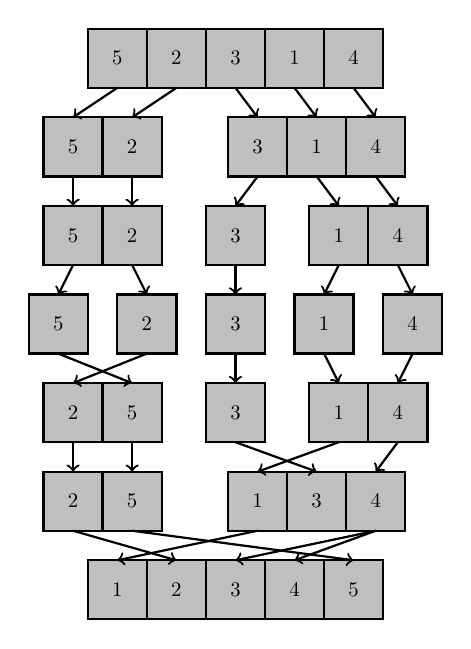
\begin{tikzpicture}[scale=0.75, transform shape]
\draw [thick, fill=gray!50] (1,9) rectangle(2,10) node[pos=.5] {5};
\draw [thick, fill=gray!50] (2,9) rectangle(3,10) node[pos=.5] {2};
\draw [thick, fill=gray!50] (3,9) rectangle(4,10)node[pos=.5] {3};
\draw [thick, fill=gray!50] (4,9) rectangle(5,10)node[pos=.5] {1};
\draw [thick, fill=gray!50] (5,9) rectangle(6,10)node[pos=.5] {4};

\draw [thick, fill=gray!50] (0.25,7.5) rectangle(1.25,8.5)node[pos=.5] {5};
\draw [thick, fill=gray!50] (1.25,7.5) rectangle(2.25,8.5)node[pos=.5] {2};
\draw [thick, fill=gray!50] (3.375,7.5) rectangle(4.375,8.5)node[pos=.5] {3};
\draw [thick, fill=gray!50] (4.375,7.5) rectangle(5.375,8.5)node[pos=.5] {1};
\draw [thick, fill=gray!50] (5.375,7.5) rectangle(6.375,8.5)node[pos=.5] {4};

\draw [thick, fill=gray!50] (0.25,6) rectangle(1.25,7)node[pos=.5] {5};
\draw [thick, fill=gray!50] (1.25,6) rectangle(2.25,7)node[pos=.5] {2};
\draw [thick, fill=gray!50] (3,6) rectangle(4,7)node[pos=.5] {3};
\draw [thick, fill=gray!50] (4.75,6) rectangle(5.75,7)node[pos=.5] {1};
\draw [thick, fill=gray!50] (5.75,6) rectangle(6.75,7)node[pos=.5] {4};

\draw [thick, fill=gray!50] (0,4.5) rectangle(1,5.5)node[pos=.5] {5};
\draw [thick, fill=gray!50] (1.5,4.5) rectangle(2.5,5.5)node[pos=.5] {2};
\draw [thick, fill=gray!50] (3,4.5) rectangle(4,5.5)node[pos=.5] {3};
\draw [thick, fill=gray!50] (4.5,4.5) rectangle(5.5,5.5)node[pos=.5] {1};
\draw [thick, fill=gray!50] (6,4.5) rectangle(7,5.5)node[pos=.5] {4};

\draw [thick, fill=gray!50] (0.25,3) rectangle(1.25,4)node[pos=.5] {2};
\draw [thick, fill=gray!50] (1.25,3) rectangle(2.25,4)node[pos=.5] {5};
\draw [thick, fill=gray!50] (3,3) rectangle(4,4)node[pos=.5] {3};
\draw [thick, fill=gray!50] (4.75,3) rectangle(5.75,4)node[pos=.5] {1};
\draw [thick, fill=gray!50] (5.75,3) rectangle(6.75,4)node[pos=.5] {4};

\draw [thick, fill=gray!50] (0.25,1.5) rectangle(1.25,2.5)node[pos=.5] {2};
\draw [thick, fill=gray!50] (1.25,1.5) rectangle(2.25,2.5)node[pos=.5] {5};
\draw [thick, fill=gray!50] (3.375,1.5) rectangle(4.375,2.5)node[pos=.5] {1};
\draw [thick, fill=gray!50] (4.375,1.5) rectangle(5.375,2.5)node[pos=.5] {3};
\draw [thick, fill=gray!50] (5.375,1.5) rectangle(6.375,2.5)node[pos=.5] {4};

\draw [thick, fill=gray!50] (1,0) rectangle(2,1)node[pos=.5] {1};
\draw [thick, fill=gray!50] (2,0) rectangle(3,1)node[pos=.5] {2};
\draw [thick, fill=gray!50] (3,0) rectangle(4,1)node[pos=.5] {3};
\draw [thick, fill=gray!50] (4,0) rectangle(5,1)node[pos=.5] {4};
\draw [thick, fill=gray!50] (5,0) rectangle(6,1)node[pos=.5] {5};
\draw [thick,draw=black,->] (3.875,1.5) -- (1.5,1);
\draw [thick,draw=black,->] (0.75,1.5) -- (2.5,1);
\draw [thick,draw=black,->] (5.875,1.5) -- (3.5,1);
\draw [thick,draw=black,->] (5.875,1.5) -- (4.5,1);
\draw [thick,draw=black,->] (1.75,1.5) -- (5.5,1);
\draw [thick,draw=black,->] (0.75,3) -- (0.75,2.5);
\draw [thick,draw=black,->] (1.75,3) -- (1.75,2.5);
\draw [thick,draw=black,->] (3.5,3) -- (4.875,2.5);
\draw [thick,draw=black,->] (5.25,3) -- (3.875,2.5);
\draw [thick,draw=black,->] (6.25,3) -- (5.875,2.5);
\draw [thick,draw=black,->] (2,4.5) -- (0.75,4);
\draw [thick,draw=black,->] (0.5,4.5) -- (1.75,4);
\draw [thick,draw=black,->] (3.5,4.5) -- (3.5,4);
\draw [thick,draw=black,->] (5,4.5) -- (5.25,4);
\draw [thick,draw=black,->] (6.5,4.5) -- (6.25,4);
\draw [thick,draw=black,->] (0.75,6) -- (0.5,5.5);
\draw [thick,draw=black,->] (1.75,6) -- (2,5.5);
\draw [thick,draw=black,->] (3.5,6) -- (3.5,5.5);
\draw [thick,draw=black,->] (5.25,6) -- (5,5.5);
\draw [thick,draw=black,->] (6.25,6) -- (6.5,5.5);
\draw [thick,draw=black,->] (0.75,7.5) -- (0.75,7);
\draw [thick,draw=black,->] (1.75,7.5) -- (1.75,7);
\draw [thick,draw=black,->] (3.875,7.5) -- (3.5,7);
\draw [thick,draw=black,->] (4.875,7.5) -- (5.25,7);
\draw [thick,draw=black,->] (5.875,7.5) -- (6.25,7);
\draw [thick,draw=black,->] (1.5,9) -- (0.75,8.5);
\draw [thick,draw=black,->] (2.5,9) -- (1.75,8.5);
\draw [thick,draw=black,->] (3.5,9) -- (3.875,8.5);
\draw [thick,draw=black,->] (4.5,9) -- (4.875,8.5);
\draw [thick,draw=black,->] (5.5,9) -- (5.875,8.5);
\end{tikzpicture}
\caption[Darstellung Merge-Sort Beispiel]{Ablauf eines Merge-Sort über ein Array aus Beispielzahlen}
\label{fig:mergesort}
\end{figure}
Um die Elemente der Datenstruktur (im Folgenden: Liste) sortieren zu können,  werden diese zunächst rekursiv geteilt.  Dafür wird die Liste in eine linke und rechte Hälfte geteilt.  Die Hälften stellen jeweils die Basis für den nächsten Teilungsschritt dar. Der Vorgang wird rekursiv wiederholt bis jede Teilliste aus genau einem Element besteht. Die Teilung der Datenelemente fordert eine vernachlässigbare Rechenleistung und hat keinen zusätzlichen Speicherbedarf. Im Anschluss wird die Rekursion der Teilung zurück durchlaufen. Hierbei findet die Sortierung statt. Die geteilten Listen werden innerhalb der Rekursion zu Zweierpaaren jeweils sortiert in eine neue Liste zusammengeführt. In der Informatik wird dabei auch von \textit{Konkatenierung} gesprochen.  Aufgrund der Zusammenführung der Listen aus zwei bereits sortierten Teillisten können im Sortiervorgang jeweils die ersten Elemente verglichen werden. Das Element mit dem niedrigeren der beiden Werte wird in die Liste der Zusammenführung gespeichert. Da in diesem Schritt zeitgleich mit drei Listen gearbeitet wird, ist zusätzlicher Speicherplatz für die Liste der sortierten Elemente nötig. Der Ablauf des \textit{merge} bzw. Zusammenführens wird bis zur Startgröße der Liste fortgeführt (s. Abbildung~\ref{fig:mergesort}). 
\\
Der maßgebliche Rechenaufwand des Algorithmus ergibt sich durch die Vergleiche zwischen den Listenelementen während der Zusammenführung. Die Laufzeit lässt sich nach der Landau-Notation darstellen. Im Vergleich zu anderen Sortieralgorithmen (z.B. Quick Sort) beträgt die Laufzeit bei Merge Sort im schlechtesten,  durschschnittlichen und besten Fall stets 
\begin{math}
\mathcal{O}(n\log n)
\end{math}.
Trotz der immer gleichen Komplexitätsklasse nach Landau-Notation wird Merge-Sort selten für die Sortierung großer Datenmengen verwendet.  Neben den Speicherzugriffen muss der zusätzlich benötigte Speicher in die Betrachtung der für die Praxis relevanten Ressourcenverbrauch einbezogen werden. Wie oben erläutert wird beim Zusammenführen der zwei Listen eine dritte Liste benötigt. Diese nimmt im letzten Konkatenierungsschritt die Länge aller Elemente an. Dementsprechend werden für Merge-Sort neben der Rechenleistung ein Speicherbedarf in Größe der Ausgangsdaten benötigt. Trotz der niedrigeren Komplexitätsklasse auch im schlechtesten Fall werden in der Praxis wegen des Speicherbedarfs meist andere Sortierverfahren ohne zusätzlichen Speicherbedarf verwendet~\cite{b3}.